\section{Problem Description}
Suppose there are $n$ voters, each voter has a certain amount of voting power $a[i],i=1,2,...,n$.

The liquid democracy refers that, each voter (called delegator) can delegate all his voting power to another voter (called delegatee), and his degegatee can further delegate all those voting power to another delegatee. Whenever a delegatee votes to a candidate, by default, all his delegators' (including multi-level) voting powers are also cast to that candidate.

We use a (direct) graph $G=(V,E)$ to represent the delegate relationship among
voters, where each note represents a voter, and a direct edge $(u,v)$
represents that voter $v$ delegates to voter $u$. Since by default there is no
loop in $G$, thus $G$ is a forest (multiple trees). For convenience, in the
case where there are more than one connect branch, we add a virtual node that
is pointed by the root of each branch. So $G$ is transferred to tree $T$, as
Figure~\ref{fig:1}.

That is, there are 12 voters, each node's  (voter) parent represents its
delegatee. As an example, now we  suppose $a[i]=i$. At the beginning, nobody
votes. When voter 1 votes for candidate $A$ (as the first voter), $A$ obtains
$1+2+...+12=78$ votes.

Meanwhile liquid democracy allows voters to change their votes when they are unsatisfied with the voting results of delegatees (including multilevel). Correspondingly, their delegatees' voting powers decrease.

As Figure~\ref{fig:1}, after voter 1 votes, suppose voter 5 (as the second
voter) votes for candidate $B$. Then $B$ obtains $6+5=11$ votes. $A$'s vote
decreases by 11, turning into 67.

Suppose further, voter 3 (the third voter) votes for candidate $C$, then $C$
obtains $3+4+7+8=22$ votes, $A$'s  vote become 45, and $B$'s vote is still 11.

\begin{figure*}
  \centering
	\label{fig:1}
	%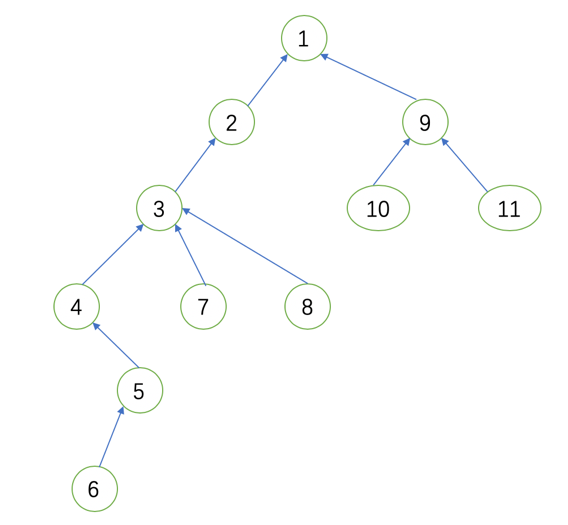
\includegraphics[width=0.6\textwidth]{1.png}
	%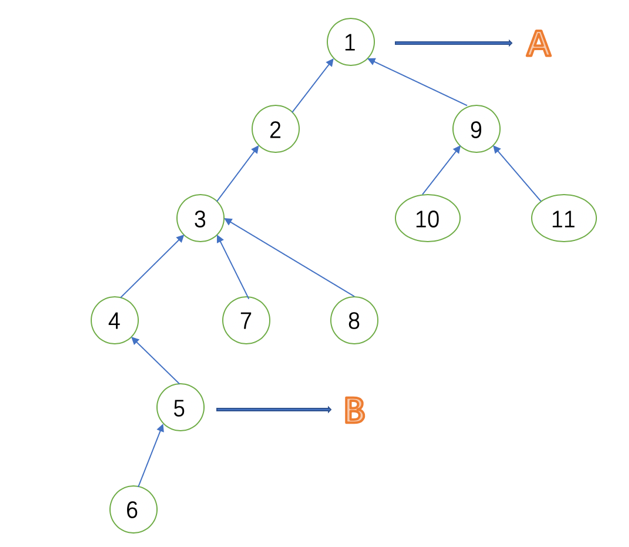
\includegraphics[width=0.6\textwidth]{2.png}
	%
  \begin{tikzpicture}
%\tikzset{grow'=right,level distance=32pt}
%\tikzset{execute at begin node=\strut}
%\tikzset{every tree node/.style={anchor=base west}}
\Tree
[.\node[fsn](n1){1};
  [.\node[sn]{2};
   [.\node[sn]{3};
    [.\node[sn]{4};
     [.\node[fsn](n5){5};
      [.\node[sn]{6};]]]
    [.\node[sn]{7};
     [.\node[sn](n8){8};]]] ]
  [.\node[sn]{9};
   [.\node[sn]{10};]
   [.\node[sn]{11};]
   [.\node[sn]{12};]]
]
\node (a) at ($(n1.east) + (1, 0)$) {A};
\node (b) at ($(n5.west) + (-1, 0)$) {B};
\draw [->, >=stealth', color=blue] (n1) -- (a);
\draw [->, >=stealth', color=blue] (n5) -- (b);

\end{tikzpicture}

	\caption{Tree $T$. We ignore the virtual node with index 0 here.}
\end{figure*}
\subsection{Goal}
Input $n<10000000,a[i],T$. Each time input a voter and a candidate that he votes, output the current voting state of all candidates (with time complexity $O(\log n)$).

Example:

\begin{tabular}{|c|c|}
input & output \\
1 A			&		A 78 B 0 C 0
\\
5 B			&		A 67 B 11 C 0
\\
3 C			&		A 45 B 11 C 22
\end{tabular}


